% Drawing 154/05-15 -- folder 154, batch 05, archive page 92 (PDF page 93).
% Transcription: petit dessin en couleur dans la note « NB » écrite en biais : une droite jaune, surchargée de points noirs, et deux croix rouges marquées $T_1$, $T_2$, l'une sur la droite, l'autre à son extrémité
% Kind: line with two red crosses T1, T2. Method 2 (schematic redraw from the facsimile). Status: ok.
% Notes: The yellow stroke runs along the slanted writing; a row of black dots is drawn over its upper half; one red cross sits on it near its lower end, the other at its upper end. The letters T_1 and T_2 are placed after the transcription (they are lost in the surrounding handwriting on the crop). Redrawn 2026-11-12 (issue 128): to check again.
% Coordinates: 1 unit = 1 mm = 1/100 of the crop width (bbox in page fractions: [0.555, 0.185, 0.655, 0.255]).
% Redrawn by Claude (claude-fable-5-2), issue #128, 2026-11-12; not checked by a human; not compiled (no TeX in the session).
% Rights: reproduces part of the work -- behind RENDER_TRANSCRIPTS, never published by itself.
\documentclass[tikz,border=3pt]{standalone}
\usepackage{amsmath,amssymb}
\usetikzlibrary{patterns,arrows.meta}
\tikzset{Ye/.style={yellow!80!orange}, Rd/.style={red!85!black}, pencil/.style={black!45}, struck/.style={black!35}, mpt/.style={circle,draw,inner sep=1.3pt}, pt/.style={circle,fill,inner sep=0.9pt}, opt/.style={circle,draw,fill=white,inner sep=1.1pt}}
\begin{document}
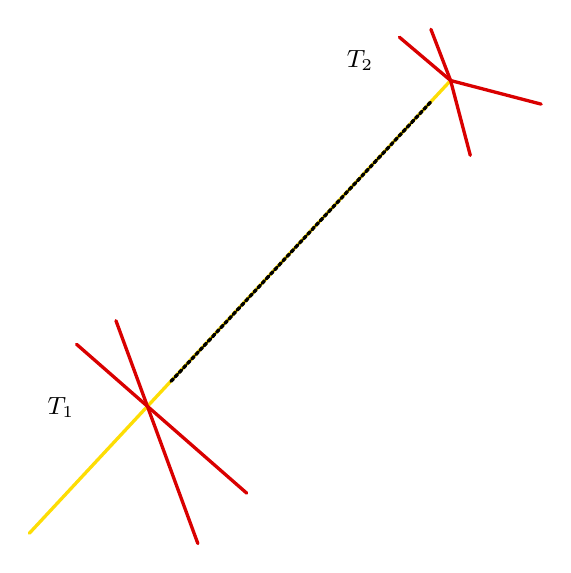
\begin{tikzpicture}[x=1mm,y=1mm,line cap=round,line join=round,font=\scriptsize]
\draw[Ye,very thick] (22,-86) -- (75.5,-28.5);
\draw[densely dotted,very thick] (40,-66.7) -- (73,-31.2);
\draw[Rd,very thick] (28,-62) -- (49.6,-80.9);
\draw[Rd,very thick] (33,-59) -- (43.4,-87.3);
\draw[Rd,very thick] (69,-23) -- (75.5,-28.5) -- (87,-31.5);
\draw[Rd,very thick] (73,-22) -- (75.5,-28.5) -- (78,-38);
\node[inner sep=1pt] at (26,-70) {\small $T_1$};
\node[inner sep=1pt] at (64,-26) {\small $T_2$};
\end{tikzpicture}
\end{document}
